\documentclass[10pt]{article}
\usepackage[english,russian]{babel}
\usepackage{textcomp}
\usepackage[left=2cm, right=2cm, top=1.5cm, bottom=1.5cm]{geometry}
\usepackage{tikz}
\usepackage{multicol}
\usepackage{hyperref}
\usepackage{amsmath}
\usepackage{listings}
\usepackage{colortbl}
\usepackage{graphicx}
\usepackage[shortlabels]{enumitem}
\usepackage{hyperref}
\pagenumbering{gobble}

\lstdefinestyle{CStyle}{
  language=C,
  basicstyle=\linespread{1.1}\ttfamily,
  basewidth=0.5em,
  texcl=true,
  keywordstyle=\color{blue}\bfseries,
  commentstyle=\color{gray},
  stringstyle=\ttfamily\color{orange!50!black},
  showstringspaces=false,
  backgroundcolor=\color{white},
  breaklines=true,
  breakatwhitespace=true,
  xleftmargin=5mm,
  keepspaces = true,
  extendedchars=\true,
  tabsize=4,
  upquote=true,
  emph={size_t, NULL},
  emphstyle={\color{blue}\bfseries},
}
\lstdefinestyle{longCodeStyle}{
  style=CStyle,
  framexleftmargin=5mm, 
  frame=shadowbox, 
  rulesepcolor=\color{gray}
}
\lstset{style=CStyle}


\renewcommand{\thesubsection}{\arabic{subsection}}
\makeatletter
\def\@seccntformat#1{\@ifundefined{#1@cntformat}%
   {\csname the#1\endcsname\quad}
   {\csname #1@cntformat\endcsname}}
\newcommand\section@cntformat{}
\newcommand\subsection@cntformat{Задача \thesubsection.\space}
\newcommand\subsubsection@cntformat{\thesubsubsection.\space}
\makeatother


\begin{document}

\title{Семинар \#3: Строки. Домашнее задание.\vspace{-5ex}}\date{}\maketitle

\subsection{Коды и символы}
Что напечатает данная программа?
\begin{lstlisting}
#include <stdio.h>
int main()
{
	printf("%i\n", '>');
	printf("%i\n", '1');
	printf("%i\n", '\0');
	printf("%i\n", '\n');
	printf("%i\n", '4' * '2');
	printf("%i\n", '7' - '0');
	printf("%c\n", 't' - 32);
	printf("%c\n", 'X' + 'a' - 'A');
}
\end{lstlisting}
Для сдачи задачи создайте в текстовом редакторе файл \texttt{01.txt}, запишите в нем все ответы, а затем добавьте файл в ваш github-репозиторий.

\subsection{Печать всех символов}
Напишите программу, которая будет печатать на экран все символы с кодами от 32 до 126 в формате:
\begin{verbatim}
    Symbol = A, Code = 65
\end{verbatim}
                

\subsection{Тип символа}
Напишите программу, которая будет считывать символ и печатать:
\begin{itemize}
\item \texttt{Letter}, если этот символ – буква (\texttt{[A, Z]} и \texttt{[a, z]})
\item \texttt{Digit}, если этот символ – цифра
\item \texttt{Other}, если это какой-то другой символ
\end{itemize}

Решите эту задачу в трёх вариантах:
\begin{enumerate}[(a)]
\item Без использования строковых литералов и библиотеки \texttt{ctype.h}
\item Используя строковые литералы, но без использования библиотеки \texttt{ctype.h}
\item Используя библиотеку \texttt{ctype.h}
\end{enumerate}



\subsection{Чередование}
Считать 2 слова и печатать их чередуя по одному символу. То есть сначала напечатать первый символ первой строки, потом первый символ второй строки, потом второй символ первой строки, второй символ второй и т. д. Если какая-то из строк закончится, то нужно допечатать оставшуюся строку.
\begin{center}
\begin{tabular}{ l | l }
 вход & выход \\ \hline
 \texttt{cat dog} & \texttt{cdaotg}  \\ 
 \texttt{cat elephant} & \texttt{cealtephant} \\
 \texttt{elephant dog} & \texttt{edloegphant} \\
 \texttt{aaaa bbbb} & \texttt{abababab} \\
 \texttt{aaaa b} & \texttt{abaaa}\\ 
 \texttt{a b} & \texttt{ab}\\ 
\end{tabular}
\end{center}


\subsection{Сумма цифр}
На вход программе поступает число из диапазона от $0$ до $10^{10^8}$. Найти сумму цифр этого числа 
\begin{center}
\begin{tabular}{ l | l }
 вход & выход \\ \hline
 \texttt{0} & \texttt{0}  \\ 
 \texttt{123} & \texttt{6} \\
 \texttt{9999999999999999999999999} & \texttt{225} \\
\end{tabular}
\end{center}


\subsection{Палиндром}
Написать функцию \texttt{is\_palindrom}, которая будет принимать строку и проверять является ли эта строка палидромом.

\begin{multicols}{2}
\begin{center}
\begin{tabular}{ l | l }
 вход & выход \\ \hline
 \texttt{abba} & \texttt{Yes} \\
 \texttt{aba} & \texttt{Yes} \\
 \texttt{a} & \texttt{Yes} \\
 \texttt{aa} & \texttt{Yes} \\
 \texttt{ab} & \texttt{No} 
\end{tabular}
\end{center}


\begin{center}
\begin{tabular}{ l | l }
 вход & выход \\ \hline
 \texttt{abcdedcba} & \texttt{Yes} \\
 \texttt{abcdedcb} & \texttt{No} \\
 \texttt{abcdedcbab} & \texttt{No} \\
 \texttt{abcdedcbb} & \texttt{No} \\
 \texttt{abcxedcba} & \texttt{No}
\end{tabular}
\end{center}
\end{multicols}


\subsection{Шифр Цезаря}
Шифр Цезаря — это вид шифра подстановки, в котором каждый символ заменяется символом, находящимся на некотором постоянном числе позиций левее или правее него в алфавите. 
\begin{center}
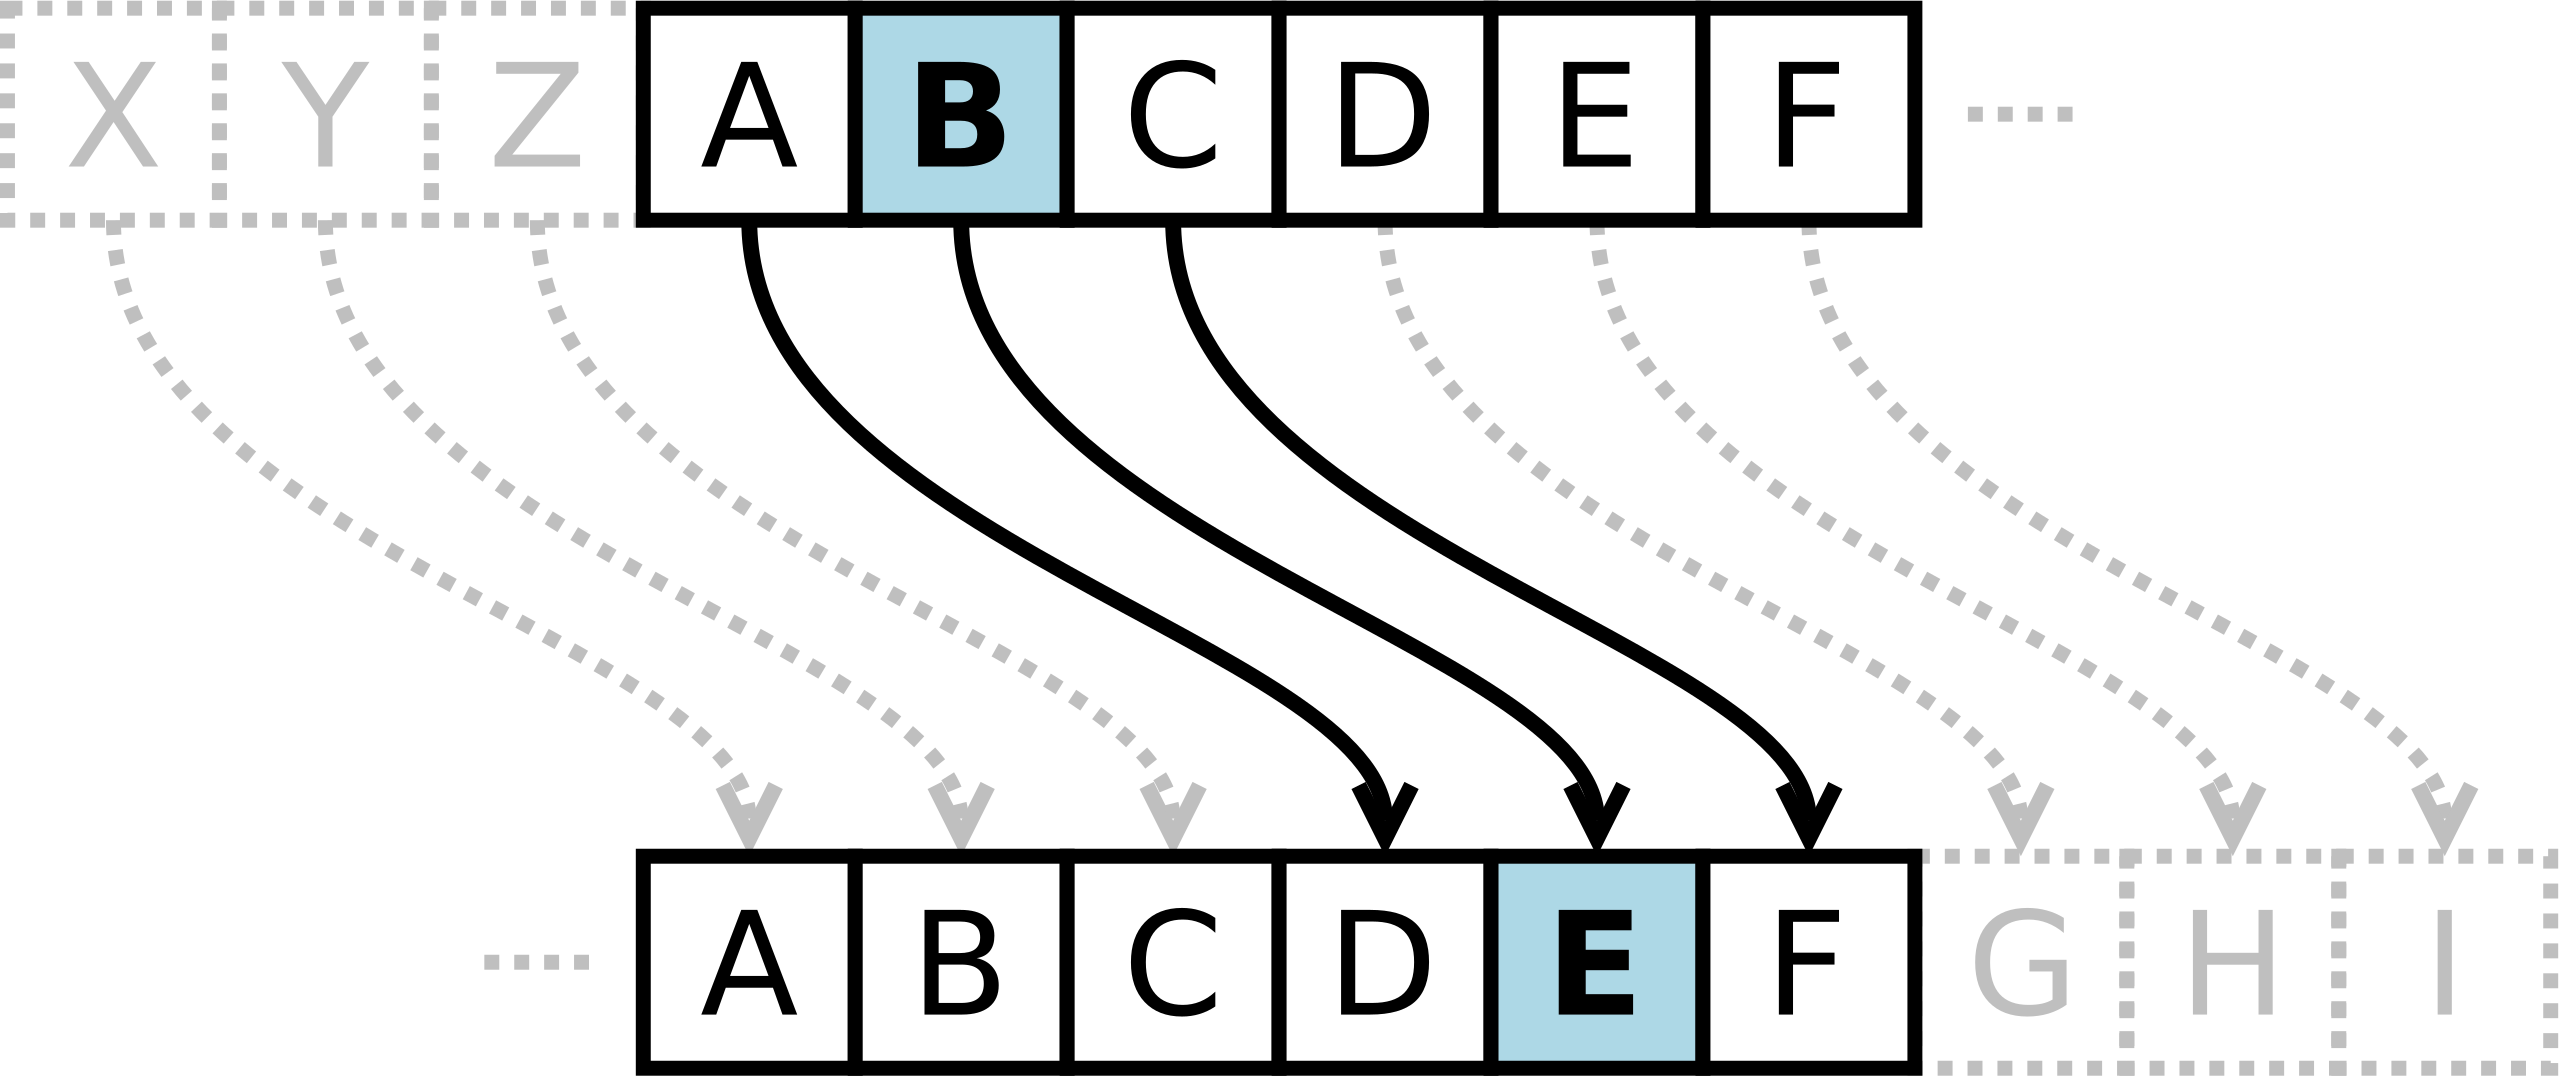
\includegraphics[width=0.4\textwidth]{../images/caesar.png}
\end{center}
Напишите функцию \texttt{void encrypt(char* str, int k)}, которая будет зашифровывать фразу шифром Цезаря.
\begin{center}
\begin{tabular}{ c | c }
 вход & выход \\ \hline
 \texttt{1 ABCZ} & \texttt{BCDA}\\
 \texttt{15 ZzZzZ} & \texttt{OoOoO} \\
 \texttt{7 The Fox Jumps Over The Dog} & \texttt{Aol Mve Qbtwz Vcly Aol Kvn} \\
 \texttt{13  Green Terra} & \texttt{Terra Green}
\end{tabular}
\end{center}


\subsection{Ошибка в считывании}
Если в этой программе ввести число, нажать \texttt{Enter} и ввести строку, то произойдёт ошибка. Почему? Исправьте эту ошибку.
\begin{lstlisting}
#include <stdio.h>
int main()
{
    int a;
    scanf("%i", &a);
    printf("a = %i\n", a);

    char str[100];
    scanf("%[^\n]", str);
    printf("str = %s\n", str);
}
\end{lstlisting}
Для сдачи задачи создайте в текстовом редакторе файл \texttt{08.txt}, запишите в нем причину ошибки и способ ее исправления, затем добавьте файл в ваш github-репозиторий.


\subsection{Укоротить строку}
Напишите функцию \texttt{void trim\_after\_first\_space(char str[])}, которая будет принимать на строку и укорачивать её до первого пробела. Протестируйте функцию с помощью следующего кода:
\begin{lstlisting}
#include <stdio.h>
// Тут вам нужно написать функцию trim\_after\_first\_space
int main() 
{
    char a[] = "Cats and Dogs";
    printf("%s\n", a); // Должно напечатать Cats and Dogs
    trim_after_first_space(a);
    printf("%s\n", a); // Должно напечатать Cats
}
\end{lstlisting}


\subsection{Сокровище}
Вы находитесь на плоскости в начале координат (точке с координатами \texttt{(0, 0)}) и вам нужно найти закопанное сокровище. Путь до него задаётся последовательностью команд, состоящих из направления и расстояния, которое нужно пройти в этом направлении. Вам нужно найти координаты сокровища. Используйте функцию \texttt{strcmp}.
\begin{center} 
\begin{tabular}{ l | l }
 вход & выход \\ \hline
 \texttt{6} & \texttt{-30 20}\\
 \texttt{North 10} & \\
 \texttt{East 20} &\\
 \texttt{South 50} &\\
 \texttt{West 60} &\\
 \texttt{East 10} &\\
 \texttt{North 60} &\\
\end{tabular}
\end{center}


\subsection{Безопасный \texttt{strcpy}}
Известно, что функция \texttt{strcpy} небезопасна, так как может выйти за границы массива, в который она записывает.
Например, в следующем примере:
\begin{lstlisting}
char a[10] = "Mouse";
char b[50] = "LargeElephant";
strcpy(a, b); // UB, выйдет за пределы массива a
\end{lstlisting}
Ваша задача заключается в том, чтобы написать функцию \texttt{safe\_strcpy}, которая будет более безопасной, чем функция \texttt{strcpy} и не будет выходить за границы массива. Эта функция должна иметь 3 параметра:
\begin{itemize}
\item строка в которую мы будем записывать (тип \texttt{char[]})
\item размер массива в который мы будем записывать (тип \texttt{size\_t})
\item строка из которой мы будем считывать (тип \texttt{const char[]}).
\end{itemize}
В случае если строка из которой мы считываем не будет помещаться в массив, нужно скопировать только часть строки, которая может поместиться в него. И обязательно поставить нулевой символ в конце строки.
\begin{lstlisting}
char a[10] = "Mouse";
char b[50] = "LargeElephant";
safe_strcpy(a, 10, b); // OK, строка a будет равна "LargeElep\textbackslash 0"
\end{lstlisting}



\subsection{Повторитель}
Напишите программу \texttt{repeater}, которая будет принимать через аргументы командной строки некоторое слово и некоторое число. Эта программа должна печатать это слово столько раз, чему равно переданное число.\\
Например, если мы вызовем эту программу так:
\begin{lstlisting}
./repeater Hello 5
\end{lstlisting}
то программа должна напечатать:
\begin{lstlisting}
Hello Hello Hello Hello Hello
\end{lstlisting}
Если вы программируете под Windows, то исполняемый файл будет называться \texttt{repeater.exe}, а не \texttt{repeater}.


\subsection{Простой калькулятор}
Напишите программу \texttt{calc}, которая будет выполнять базовые арифметические операции над двумя целыми числами. Программа должна принимать строго 3 аргумента командной строки (при этом \texttt{argc} будет иметь значение 4) в следующем порядке:
\begin{itemize}
\item Первый операнд
\item Знак оператора (\texttt{+}, \texttt{-}, \texttt{*}, \texttt{/} или \texttt{\%})
\item Второй операнд
\end{itemize}
Команда должна поддерживать: сложение, вычитание, умножение, целочисленное деление и нахождение остатка. Программа должна обрабатывать такие ошибки во входных данных, как неверное количество аргументов, неверный оператор, неверный формат операндов и ошибку деления на ноль. \\
Примеры использования программы:
\begin{lstlisting}
$ ./calc 10 + 20
30

$ ./calc 500 / 9
55

$ ./calc 11 * 12
132

$ ./calc 20 % 7
6

$ ./calc 5
Error: Wrong number of arguments!
Usage: ./calc <number> <operator> <number>

$ ./calc 10 & 20
Error: Invalid operator!

$ ./calc 10.5 + abc
Error: Operands should be integers!

$ ./calc 10 / 0
Error: Division by zero!
\end{lstlisting}
Если вы программируете под Windows, то исполняемый файл будет называться \texttt{calc.exe}, а не \texttt{calc}.


\subsection{Шифрование файла}
Напишите программу \texttt{encrypt}, которая будет принимать через аргументы командной строки названия входного и выходного файлов, а также число-ключ шифра Цезаря. Программа должна считывать входной файл, зашифровывать его шифром Цезаря и записывать результат в выходной файл.\\
Например, если мы вызовем эту программу так:
\begin{verbatim}
./encrypt a.txt b.txt 7
\end{verbatim}
то программа должна считывать файл \texttt{a.txt}, зашифровывать содержимое шифром Цезаря с ключом 7 и записывать результат в файл \texttt{b.txt}. В данной задаче необязательно обрабатывать ошибки во входных данных.\\
Проверьте работу программы на файлах \texttt{three\_little\_pigs.txt} и \texttt{invisible\_man.txt}.

\noindent Если вы программируете под Windows, то исполняемый файл будет называться \texttt{encrypt.exe}, а не \texttt{encrypt}.


\subsection{Извлечение строк}
Напишите программу \texttt{line\_extractor}, которая будет извлекать строки из файла. Программа должна принимать строго 3 аргумента командной строки:
\begin{itemize}
\item Имя входного файла
\item Имя нового файла, который будет содержать определённые строки
\item Или одно число -- номер строки, или диапазон строк в формате \texttt{начало:конец}
\end{itemize}

\noindent Например, если вызвать программу так:
\begin{lstlisting}
$ ./line_extractor a.txt b.txt 10
\end{lstlisting}
то она должна создать новый файл \texttt{b.txt} и поместить туда 10-ю строку из файла \texttt{a.txt}.\\

\noindent Если же вызвать программу так:
\begin{lstlisting}
$ ./line_extractor a.txt b.txt 10:20
\end{lstlisting}
то программа должна создать новый файл \texttt{b.txt} и поместить туда строки из 10-й по 20-ю (не включительно) из файла \texttt{a.txt}.\\

\noindent Если аргументы заданы неверно, то программа должна напечатать сообщение о ошибке и завершиться. Программа должна обрабатывать следующие ошибки:
\begin{itemize}
\item Неверное количество аргументов
\item Начальный файл не существует.
\item Неверный формат задания номера строки или диапазона строк.
\end{itemize}
Примеры ошибочных вызовов программы:
\begin{lstlisting}
$ ./line_extractor result.txt
Error: Wrong number of arguments!
Usage: ./line_extractor <input_file> <output_file> <lines

$ ./line_extractor qwertyuiop.txt b.txt 10
Error: File qwertyuiop.txt does not exist!

$ ./line_extractor a.txt b.txt 10:20abc
Error: Wrong lines format!

$ ./line_extractor a.txt b.txt 10:
Error: Wrong lines format!
\end{lstlisting}
Проверьте работу программы на файлах \texttt{three\_little\_pigs.txt} и \texttt{invisible\_man.txt}.


\noindent Если вы программируете под Windows, то исполняемый файл будет называться \texttt{line\_extractor.exe}, а не \texttt{line\_extractor}.



\newpage
~
\newpage
\section*{Необязательные задачи (не входят в ДЗ, никак не учитываются)}
\setcounter{subsection}{0}

\subsection{Номер буквы}
Считайте символ буквы латинского алфавита и напечатайте его номер в алфавите. Если на вход подаётся не буква, то нужно напечатать \texttt{Not a letter}.
\begin{center}
\begin{tabular}{ l | l }
 вход & выход \\ \hline
 \texttt{P} & \texttt{16} \\
 \texttt{b} & \texttt{2} \\
 \texttt{B} & \texttt{2} \\
 \texttt{\#} & \texttt{Not a letter}\\ 
\end{tabular}
\end{center}

\subsection{Лесенка}
Считать слово и напечатать лесенку из этого числа. Например, для слова \texttt{Hello} нужно напечатать лесенку: 
\begin{center}
\begin{center}
\begin{tabular}{ c | l }
 вход & выход \\ \hline
 \texttt{Hello} & \texttt{H}  \\ 
 & \texttt{He} \\
 & \texttt{Hel} \\
 & \texttt{Hell} \\
 & \texttt{Hello}\\ 
\end{tabular}
\end{center}
\end{center}



\subsection{Восклицание}
На вход подаётся строка. Напечатать эту же строку, но ставя восклицательный знак после каждого слова.
\begin{center}
\begin{tabular}{ l | l }
 вход & выход \\ \hline
 \texttt{Better late than never} & \texttt{Better! late! than! never!} \\
 \texttt{cat \quad dog elephant} & \texttt{cat! \quad dog! elephant!}  \\ 
 \texttt{a} & \texttt{a!} \\
\end{tabular}
\end{center}


\subsection{Правильная скобочная последовательность}
На вход подаётся скобочная последовательность(строка, состоящая из символов \texttt{'('} и \texttt{')'}). Нужно выяснить является ли эта скобочная последовательность допустимой или нет.
\begin{multicols}{2}
\begin{center}
\begin{tabular}{ l | l }
 вход & выход \\ \hline
 \texttt{(()())} & \texttt{Yes} \\
 \texttt{(()(()()))} & \texttt{Yes} \\
 \texttt{(()))()())} & \texttt{No} \\
 \texttt{(((())))} & \texttt{Yes} \\
 \texttt{(((()))))} & \texttt{No} \\
 \texttt{(((()))} & \texttt{No} \\
\end{tabular}
\end{center}

\begin{center}
\begin{tabular}{ l | l }
 вход & выход \\ \hline
 \texttt{()} & \texttt{Yes} \\
 \texttt{)(} & \texttt{No} \\
 \texttt{))} & \texttt{No} \\
 \texttt{((} & \texttt{No} \\
 \texttt{()()} & \texttt{Yes} \\
 \texttt{(} & \texttt{No} \\
 \texttt{)} & \texttt{No} \\
\end{tabular}
\end{center}
\end{multicols}


\subsection{Удаление символа}
Напишите функцию \texttt{void delete\_chars(char str[], char c)}, которая будет удалять все символы, равные \texttt{c} из строки \texttt{str}. Постарайтесь сделать эту функцию как можно более эффективной.

\begin{center}
\begin{tabular}{ l | l }
 \texttt{str, c} & \texttt{str} после вызова \texttt{delete\_chars(str, c)} \\ \hline
 \texttt{cat a} & \texttt{ct} \\
 \texttt{elephant e} & \texttt{lphant} \\
 \texttt{aaaa a} & \texttt{} \\
 \texttt{a a} & \texttt{} \\
 \texttt{ababababa a} & \texttt{bbbb} \\
\end{tabular}
\end{center}


\subsection{Самое длинное слово}
Напишите функцию \texttt{int longest\_word(const char str[], char result[])}, которая будет искать самое длинное слово в строке \texttt{str} и записывать его в строке \texttt{result}. Строка должна возвращать длину этого слова. Под словом тут понимается последовательность непробельных символов, ограниченная с двух сторон пробельными символами или границами строки.
В случае если есть несколько слов с самой большой длиной в \texttt{result} нужно записать первое из них.

\begin{center}
\begin{tabular}{ l | l }
 \texttt{str} & \texttt{result} после вызова \texttt{longest\_word(str, result)} \\ \hline
 \texttt{cats and dogs} & \texttt{cats} \\
 \texttt{cat dog elephant mouse} & \texttt{elephant} \\
 \texttt{cat \quad dog \quad\quad elephant mouse} & \texttt{elephant} \\
\end{tabular}
\end{center}

\subsection{Переворот слов в файле}
Счмтайте файл \texttt{input.txt}  и переверните все слова из этого файла и запишите результат в файл \texttt{output.txt}.
\begin{center} 
\begin{tabular}{ l | l }
 файл \texttt{input.txt} & файл \texttt{output.txt} \\ \hline
 \texttt{Cat and Dog} & \texttt{taC dna goD}\\
\end{tabular}
\end{center}
Протестируйте программу на файле \texttt{invisible\_man.txt}.


\subsection{Сортировка аргументов}
Напишите программу \texttt{sort}, которая будет принимать через аргументы командной строки произвольное число строк и сортировать эти строки лексикографически и печатать их.\\
Например, если мы вызовем эту программу так:
\begin{verbatim}
./sort cat elephant mouse axolotl lion
\end{verbatim}
то программа должна напечатать:
\begin{verbatim}
axolotl cat elephant lion mouse
\end{verbatim}




\subsection{*Замена}
Напишите программу \texttt{replacer}, которая будет принимать через аргументы командной строки названия входного и выходного файлов, а также две строки. Программа должна считывать входной файл, заменять все вхождения первой строки на вторую строку и записывать результат в выходной файл.\\
Например, если мы вызовем эту программу так:
\begin{verbatim}
./replacer three_little_pigs.txt result.txt pig elephant
\end{verbatim}
то программа должна считывать файл \texttt{three\_little\_pigs.txt}, заменять все подстроки \texttt{"pig"} на \texttt{"elephant"} и записывать результат в файл \texttt{result.txt}. Постарайтесь написать эффективный алгоритм замены. Рассмотите случаи когда подстрока заменяется на более длинную строку и когда подстрока заменяется на более короткую строку.

\end{document}